\begin{savequote}[45mm]
\ascii{Any fool can write code that a computer can understand. Good programmers write code that humans can understand.}
\qauthor{\ascii{- Martin Flower}}
\end{savequote}

\chapter{物理设计} 
\label{ch:physical-design}

\section{概念}

\begin{content}

物理设计主要是软件设计中的物理实体(文件)的设计,例如某个函数定义应该放在哪个文件中、某个函数是否需要\ascii{inline}等;逻辑设计主要针对软件设计中的逻辑实体关系的设计,例如类之间的关系,\ascii{has-a/use-a/is-a}的关系。

物理设计的主要目标是减少文件的物理依赖;而逻辑设计的主要目标是减少逻辑依赖。物理依赖更多的体现为编译时的依赖和链接时的依赖;物理依赖受逻辑依赖影响,但是又不局限于逻辑依赖。

\end{content}

\section{物理结构}

\begin{content}

\begin{regulation}
遵循惯例优于配置的基本原则,公司内部所有项目组织结构应该保持一致,便于项目的自动化构建。
\end{regulation}

以\ascii{cut}项目为例,总体上分\ascii{include, src, test}三个目录;头文件,源文件,测试文件存在对称关系;构建文件分级构建,例如`CMakeLists.txt, Makefile`。

正例:
\begin{leftbar}
\begin{c++}[caption={项目结构}]
cut
├── CMakeLists.txt
├── LICENSE
├── README.md
├── include
│   └── cut
│       ├── core
│       │   ├── Test.h
│       │   ├── TestCase.h
│       │   ├── TestFixture.h
│       │   ├── TestListener.h
│       │   ├── TestResult.h
│       │   ├── TestRunner.h
│       │   └── TestSuite.h
│       ├── cut.h
│       ├── cut.hpp
├── src
│   ├── CMakeLists.txt
│   └── cut
│       ├── core
│       │   ├── TestCase.cpp
│       │   ├── TestResult.cpp
│       │   ├── TestRunner.cpp
│       │   └── TestSuite.cpp
└── test
    ├── CMakeLists.txt
    ├── cut
    │   ├── TestCaseSpec.cpp
    │   ├── TestSuiteSpec.cpp    
    │   ├── TestListenerSpec.cpp
    ├── main.cpp
\end{c++}
\end{leftbar}

\begin{regulation}
文件布局,团队应遵循统一的风格。
\end{regulation}

一个头文件包括头文件保护宏,\ascii{include}语句,命名空间,前置声明,类定义等。

正例:
\begin{leftbar}
\begin{c++}[caption={\ttfamily{cut/core/TestCase.h}}]
#ifndef _YILL50M2RW1ONKOTDE31GYE4PZNVDLHH1CKFXS75LL4DA2NDCQSX9H5Y               
#define _YILL50M2RW1ONKOTDE31GYE4PZNVDLHH1CKFXS75LL4DA2NDCQSX9H5Y

#include <cut/core/Test.h>
#include <cut/core/TestFixture.h>

CUT_NS_BEGIN

struct TestCase : Test, TestFixture
{
    TestCase(const std::string& name);

    void runBare(TestResult&);

private:
    OVERRIDE(void run(TestResult&));
    OVERRIDE(int countTestCases() const);
    OVERRIDE(int countChildTests() const);
    OVERRIDE(const std::string& getName() const);

private:
    DEFAULT(void, runTest());

private:
    template <typename Functor>
    bool protect(TestResult& result, Functor functor, const char* desc = "");

private:
    const std::string name;
};

CUT_NS_END

#endif
\end{c++}
\end{leftbar}

实现文件的布局,包括匿名命名空间定义,类成员函数实现等等。

正例:
\begin{leftbar}
\begin{c++}[caption={\ttfamily{cut/core/TestCase.cpp}}]
#include <cut/core/TestCase.h>
#include <cut/core/TestFunctor.h>
#include <cut/core/TestResult.h>

CUT_NS_BEGIN

TestCase::TestCase(const std::string& name) : name(name)
{}

namespace
{
    struct TestCaseFunctor : TestFunctor
    {
        using Method = void(TestCase::*)();
        
        TestCaseFunctor(TestCase& test, Method method)
            : test(test), method(method)
        {}

    private:
        OVERRIDE(bool operator()() const)
        {
            (test.*method)();
            return true;
        }

        IMPL_ROLE_WITH_OBJ(Test, test);

    private:
       TestCase& test;
       Method method;
    };
}

template <typename Functor>
inline bool TestCase::protect(TestResult& result, Functor functor, const char* desc)
{
    return result.protect(TestCaseFunctor(*this, functor), desc);
}

#define PROTECT(functor) protect(result, &TestCase::functor, " in the "#functor)

void TestCase::runBare(TestResult& result)
{
    if (PROTECT(setUp))
    {
        PROTECT(runTest);
    }
    PROTECT(tearDown);
}

void TestCase::run(TestResult& result)
{
    result.run(*this);
}

int TestCase::countTestCases() const
{
  return 1;
}

int TestCase::countChildTests() const
{
    return 0;
}

const std::string& TestCase::getName() const
{
    return name;
}

CUT_NS_END
\end{c++}
\end{leftbar}

实现文件是一种典型的隐藏实现的技术,能够极大地缩小用户依赖的范围,为此我们鼓励实现的隐藏和封装。例如,\ascii{TestCase::protect}虽然是模板,但它仅仅被\ascii{TestCase::runBare}所范围,为此在头文件中将其声明为\ascii{private},并且没有在头文件中展开实现。

\begin{leftbar}
\begin{c++}[caption={\ttfamily{cut/core/TestCase.h}}]
struct TestCase : Test, TestFixture
{
   ...

private:
    template <typename Functor>
    bool protect(TestResult& result, Functor functor, const char* desc = "");
};
\end{c++}
\end{leftbar}

而只需在实现文件中,在被依赖的点之前完成模板的定义即可;并且在定义时,因为在实现文件内部,所以可以大胆地使用\ascii{inline}机制。

\begin{leftbar}
\begin{c++}[caption={\ttfamily{cut/core/TestCase.cpp}}]
template <typename Functor>
inline bool TestCase::protect(TestResult& result, Functor functor, const char* desc)
{
    return result.protect(TestCaseFunctor(*this, functor), desc);
}

#define PROTECT(functor) protect(result, &TestCase::functor, " in the "#functor)

void TestCase::runBare(TestResult& result)
{
    if (PROTECT(setUp))
    {
        PROTECT(runTest);
    }
    PROTECT(tearDown);
}
\end{c++}
\end{leftbar}

\end{content}

\section{头文件}

\begin{content}

\begin{regulation}
自定义头文件必须具有扩展名,以区分\ascii{C++}标准库的头文件;在团队内部,头文件、源文件扩展名类型必须保持一致性。
\end{regulation}

表\reftbl{file-extension}列出了头文件和实现文件常见的扩展名,团队应该选择一类扩展名并保持团队内一致性。

\begin{table}[!htb]
\resizebox{0.95\textwidth}{!} {
\begin{tabular*}{1.2\textwidth}{@{}ll@{}}
\toprule
\ascii{文件类型} & \ascii{支持的扩展名} \\
\midrule
\ascii{头文件}  & \ascii{.h, .hpp, .hxx, .hh, h++, .tcc} \\
\ascii{源文件} & \ascii{.c, .C, .cpp, .cxx, .cc, .c++} \\ 
\bottomrule
\end{tabular*}
}
\caption{扩展名}
\label{tbl:file-extension}
\end{table}

\begin{regulation}
每一个头文件都应该具有独一无二的保护宏,并保持命名规则的一致性
\end{regulation}

命名规则包括两种风格:
\begin{enum}
  \eitem{INCL\_<PROJECT>\_<MODULE>\_<FILE>\_H}
  \eitem{\ascii{全局唯一的随机序列码\footnote{例如\ascii{Eclipse}可以配置头文件的代码模板,其他\ascii{IDE}也存在类似的功能。}}}
\end{enum}

第一种命名规则问题在于:当文件名重命名或移动目录时,需要同步修改头文件保护宏;推荐使用\ascii{IDE}随机自动地生成头文件保护宏,其更加快捷、简单、安全、有效。

反例:
\begin{leftbar}
\begin{c++}[caption={\ttfamily{cub/thread/Runnable.h}}]
// 因名称太短,存在名字冲突的可能性
#ifndef RUNNABLE_H
#define RUNNABLE_H

#include <cub/base/Role.h>

DEFINE_ROLE(Runnable)
{
    ABSTRACT(void run());
};

#endif
\end{c++}
\end{leftbar}

正例:
\begin{leftbar}
\begin{c++}[caption={\ttfamily{cub/thread/Runnable.h}}]
// UUID: IDE自动生成
#ifndef ADCM_LLL_3465_DCPOE_ACLDDDE_479_YTEY_SDJWEOX_234798SDN
#define ADCM_LLL_3465_DCPOE_ACLDDDE_479_YTEY_SDJWEOX_234798SDN

#include <cub/base/Role.h>

DEFINE_ROLE(Runnable)
{
    ABSTRACT(void run());
};

#endif
\end{c++}
\end{leftbar}

\begin{regulation}
包含头文件时,统一使用尖括号。
\end{regulation}

即使在同一目录下,也不采用相对路径包含头文件。这样做,在没有严重牺牲编译效率的前提下,可以形成同一的代码规范,程序员再也不用被这件事情所困扰。

反例:
\begin{leftbar}
\begin{c++}[caption={\ttfamily{cut/core/TestCase.h}}]
#ifndef _YILL50M2RW1ONKOTDE31GYE4PZNVDLHH1CKFXS75LL4DA2NDCQSX9H5Y               
#define _YILL50M2RW1ONKOTDE31GYE4PZNVDLHH1CKFXS75LL4DA2NDCQSX9H5Y

// 即使TestCase, Test, TestFixture在同一目录,
// 也不采用相对路径的方式组织include语句
#include "Test.h"
#include "TestFixture.h"

CUT_NS_BEGIN

struct TestCase : Test, TestFixture
{
    TestCase(const std::string& name);

private:
    OVERRIDE(void run(TestResult&));
    OVERRIDE(int countTestCases() const);
    OVERRIDE(int countChildTests() const);
    OVERRIDE(const std::string& getName() const);

private:
    const std::string name;
};

CUT_NS_END

#endif
\end{c++}
\end{leftbar}

正例:
\begin{leftbar}
\begin{c++}[caption={\ttfamily{cut/core/TestCase.h}}]
#ifndef _YILL50M2RW1ONKOTDE31GYE4PZNVDLHH1CKFXS75LL4DA2NDCQSX9H5Y               
#define _YILL50M2RW1ONKOTDE31GYE4PZNVDLHH1CKFXS75LL4DA2NDCQSX9H5Y

// 统一采用:#include <project/module/file.h>的风格
#include <cut/core/Test.h>
#include <cut/core/TestFixture.h>

CUT_NS_BEGIN

struct TestCase : Test, TestFixture
{
    TestCase(const std::string& name);

private:
    OVERRIDE(void run(TestResult&));
    OVERRIDE(int countTestCases() const);
    OVERRIDE(int countChildTests() const);
    OVERRIDE(const std::string& getName() const);

private:
    const std::string name;
};

CUT_NS_END

#endif
\end{c++}
\end{leftbar}

\begin{regulation}
文件名应该与程序主要实体名称相同。
\end{regulation}

反例:
\begin{leftbar}
\begin{c++}[caption={\ttfamily{cut/core/test\_case.h}}]
// 文件名与类名不一致
struct TestCase
{
    explicit TestCase(const std::string& name);

private:
    const std::string name;
};
\end{c++}
\end{leftbar}

正例:
\begin{leftbar}
\begin{c++}[caption={\ttfamily{cut/core/TestCase.h}}]
struct TestCase
{
    explicit TestCase(const std::string& name);

private:
    const std::string name;
};
\end{c++}
\end{leftbar}

\begin{regulation}
路径名一律使用小写、下划线或中划线风格的名称。
\end{regulation}

反例:
\begin{leftbar}
\begin{c++}[caption={驼峰风格的路径名}]
// 路径名\ascii{htmlParser}使用了驼峰命名风格
#include <htmlParser/core/Attribute.h>
\end{c++}
\end{leftbar}

正例:
\begin{leftbar}
\begin{c++}[caption={正确的头文件包含}]
#include <html-parser/core/Attribute.h>
\end{c++}
\end{leftbar}

\begin{regulation}
包含头文件时,必须保持路径名、文件名大小写敏感
\end{regulation}

为了保证代码的最大化可移植性,在包含头文件时必须保持文件名的大小写敏感。

假如存在两个物理文件名,真实的路径分别为:\ascii{cub/base/SynchronizedObject.h, ymal/yaml\_parser.h}。

反例:
\begin{leftbar}
\begin{c++}
// 路径名大小写与真实物理路径不符
#include <Cub/Base/SynchronizedObject.h>

// 文件名大小写与真实物理文件名称不符
#include <ymal/YAML_Parser.h>
\end{c++}
\end{leftbar}

正例:
\begin{leftbar}
\begin{c++}
#include <cut/core/SynchronizedObject.h>
#include <yaml_parser.h>
\end{c++}
\end{leftbar}

\begin{regulation}
包含头文件时,路径分隔符一律使用\ascii{Unix}风格,拒绝使用\ascii{Windows}风格。
\end{regulation}

反例:
\begin{leftbar}
\begin{c++}
// 使用了Windows风格的路径分割符
#include <cub\base\SynchronizedObject.h>
\end{c++}
\end{leftbar}

正例:
\begin{leftbar}
\begin{c++}
// 使用了Unix风格的路径分割符
#include <cub/base/SynchronizedObject.h>
\end{c++}
\end{leftbar}

\begin{regulation}
使用\ascii{extern} \texttt{"}\ascii{C}\texttt{"}时,不要包括\ascii{include}语句
\end{regulation}

反例:
\begin{leftbar}
\begin{c++}[caption={\ttfamily{oss/oss\_memery.h}}]
#ifndef HF0916DFB_1CD1_4811_B82B_9B8EB1A007D8
#define HF0916DFB_1CD1_4811_B82B_9B8EB1A007D8
    
#ifdef  __cplusplus
extern "C" {
#endif

// 错误地将include放在了extern "C"中
#include <oss/def.h>

void* oss_alloc(size_t);
void  oss_free(void*);

#ifdef  __cplusplus
}
#endif

#endif
\end{c++}
\end{leftbar}

正例:
\begin{leftbar}
\begin{c++}[caption={\ttfamily{oss/oss\_memery.h}}]
#ifndef HF0916DFB_1CD1_4811_B82B_9B8EB1A007D8
#define HF0916DFB_1CD1_4811_B82B_9B8EB1A007D8
    
#include <oss/def.h>

#ifdef  __cplusplus
extern "C" {
#endif

void* oss_alloc(size_t);
void  oss_free(void*);

#ifdef  __cplusplus
}
#endif

#endif
\end{c++}
\end{leftbar}

\begin{regulation}
当以\ascii{C}提供实现时,头文件中必须使用\ascii{extern}
\texttt{"}\ascii{C}\texttt{"}声明,以便支持\ascii{C++}的扩展。
\end{regulation}

反例:
\begin{leftbar}
\begin{c++}[caption={oss/oss\_memery.h}]
#ifndef HF0916DFB_1CD1_4811_B82B_9B8EB1A007D8
#define HF0916DFB_1CD1_4811_B82B_9B8EB1A007D8    

#include <oss/def.h>

void* oss_alloc(size_t);
void  oss_free(void*);

#endif
\end{c++}
\end{leftbar}

正例:
\begin{leftbar}
\begin{c++}[caption={oss/oss\_memery.h}]
#ifndef HF0916DFB_1CD1_4811_B82B_9B8EB1A007D8
#define HF0916DFB_1CD1_4811_B82B_9B8EB1A007D8    

#include <oss/def.h>

#ifdef  __cplusplus
extern "C" {
#endif

void* oss_alloc(size_t);
void  oss_free(void*);

#ifdef  __cplusplus
}
#endif

#endif
\end{c++}
\end{leftbar}

可以使用实用宏,消除代码重复。

正例:
\begin{leftbar}
\begin{c++}[caption={\ttfamily{oss/oss\_memery.h}}]
#ifndef HF0916DFB_1CD1_4811_B82B_9B8EB1A007D8
#define HF0916DFB_1CD1_4811_B82B_9B8EB1A007D8
    
#include <oss/def.h>
#include <cub/base/ExternC.h>

EXTERN_STDC_BEGIN

void* oss_alloc(size_t);
void  oss_free(void*);

EXTERN_STDC_END

#endif
\end{c++}
\end{leftbar}

其中,

\begin{leftbar}
\begin{c++}[caption={\ttfamily{cub/base/ExternC.h}}]
#ifndef HF90C74A1_842B_49B0_8B86_4A2A23AE28C3
#define HF90C74A1_842B_49B0_8B86_4A2A23AE28C3

#ifdef __cplusplus
    #define EXTERN_STDC_BEGIN extern "C" {
    #define EXTERN_STDC_END  }
#else
    #define EXTERN_STDC_BEGIN
    #define EXTERN_STDC_END
#endif

#endif
\end{c++}
\end{leftbar}

\begin{advise}
拒绝创建巨型头文件,将所有实体声明都放到头文件中。
\end{advise}

不要把所有的宏、\ascii{const}常量、函数声明、类定义都要放在头文件中,而仅仅将外部依赖的实体声明放到头文件中。实现文件也是一种信息隐藏的惯用技术,如果一些程序的实体不对外所依赖,则放在自己的实现文件中,一则可降低依赖关系,二则实现更好的信息隐藏。

巨型头文件必然造成了巨大的编译时依赖,不仅仅带来巨大的编译时开销,更重要的是这样的设计将太多的实现细节暴露给用户,导致后续版本兼容性的问题,阻碍了头文件进一步演进、修改、扩展的可能性,从而失去了软件的可扩展性。

不要认为提供一个大而全的头文件会给你的用户带来方便,用户因此而更加困扰。另外,头文件应该自满足,而不是让用户还要关心头文件之间的依赖关系。巨大的头文件,因为复杂,是很难保证其自满足性,从而带来维护上的麻烦,并且降低了代码的可读性。

\end{content}

\section{物理设计原则}

\begin{content}

物理设计是\clang{}\ascii{/}\cpp{}语言中特有的一部分,遵循\reftbl{phyical-design-priciples}中所列的设计原则,必然可以得到更加清晰、更加漂亮的头文件设计。

\begin{table}[!htb]
\resizebox{0.95\textwidth}{!} {
\begin{tabular*}{1.2\textwidth}{@{}ll@{}}
\toprule
\ascii{原则} & \ascii{基本含义} \\
\midrule
\ascii{自满足原则}  & \ascii{头文件本身是可以编译通过的} \\
\ascii{单一职责原则} & \ascii{头文件包含的实体的职责是单一的} \\ 
\ascii{最小依赖原则} & \ascii{绝不包含不必要的头文件} \\
\ascii{最小可见性原则} & \ascii{尽量封装隐藏类的成员} \\
\bottomrule
\end{tabular*}
}
\caption{物理设计原则}
\label{tbl:phyical-design-priciples}
\end{table}


\begin{principle}
自满足原则
\end{principle}

所有头文件都应该自满足的。所谓头文件自满足,即头文件自身是可编译成功的。

看一个具体的示例代码,这里定义了一个\ascii{TestCase.h}头文件。\ascii{TestCase}对父类\ascii{TestLeaf,
TestFixture}都存在编译时依赖,但没有包含基类的头文件。

反例:
\begin{leftbar}
\begin{c++}[caption={\ttfamily{cut/core/TestCase.h}}]
#ifndef EOPTIAWE_23908576823_MSLKJDFE_0567925
#define EOPTIAWE_23908576823_MSLKJDFE_0567925    

struct TestCase : TestLeaf, TestFixture
{
    TestCase(const std::string &name="");
    
private:
    OVERRIDE(void run(TestResult *result));
    OVERRIDE(std::string getName() const);

private:
    ABSTRACT(void runTest());
    
private:
    const std::string name;
};

#endif
\end{c++}
\end{leftbar}

为了满足自满足原则,其自身必须包含其所有父类的头文件。

正例:
\begin{leftbar}
\begin{c++}[caption={\ttfamily{cut/core/TestCase.h}}]
#ifndef EOPTIAWE_23908576823_MSLKJDFE_0567925
#define EOPTIAWE_23908576823_MSLKJDFE_0567925    

#include <cut/core/TestLeaf.h>
#include <cut/core/TestFixture.h>

struct TestCase : TestLeaf, TestFixture
{
    TestCase(const std::string &name="");
    
private:
    OVERRIDE(void run(TestResult &result));
    OVERRIDE(std::string getName() const);

private:
    ABSTRACT(void runTest());
    
private:
    const std::string name;
};

#endif
\end{c++}
\end{leftbar}

即使\ascii{TestCase}持有\ascii{std::string name}成员变量,但没有必要包含\ascii{std::string}的头文件。因为\ascii{TestCase}覆写了其父类的\ascii{getName}成员函数,父类为了保证自满足原则,自然已经包含了\ascii{std::string}的头文件。

同样的原因,也没有必要在此前置声明\ascii{TestResult},因为父类已经声明过了。两者成立的前提时,父类都要遵循良好的头文件自满足原则。

\begin{regulation}
实现文件的第一行代码必然是包含其对应的头文件。
\end{regulation}

创建对应的实现文件\ascii{TestCase.cpp},并将自身头文件的进行包含,并置在实现文件的第一行,这是验证头文件自满足的最好的办法。

反例:
\begin{leftbar}
\begin{c++}[caption={\ttfamily{cut/core/TestCase.cpp}}]
#include <cut/core/TestResult.h>
#include <cut/core/Functor.h>
// 没有放在第一行,无法校验其自满足性
#include <cut/core/TestCase.h>

namespace
{
    struct TestCaseMethodFunctor : Functor
    {
        typedef void (TestCase::*Method)();
    
        TestCaseMethodFunctor(TestCase &target, Method method)
           : target(target), method(method)
        {}
    
        bool operator()() const
        {
            target.*method();
            return true;
        }
    
    private:
        TestCase &target;
        Method method;
    };
}

template <typename Functor>
inline bool TestCase::protect(TestResult& result, Functor functor, const char* desc)
{
    return result.protect(TestCaseFunctor(*this, functor), desc);
}

#define PROTECT(functor) protect(result, &TestCase::functor, " in the "#functor)

void TestCase::runBare(TestResult& result)
{
    if (PROTECT(setUp))
    {
        PROTECT(runTest);
    }
    PROTECT(tearDown);
}
...

\end{c++}
\end{leftbar}

正例:
\begin{leftbar}
\begin{c++}[caption={\ttfamily{cut/core/TestCase.cpp}}]
#include <cut/core/TestCase.h>
#include <cut/core/TestResult.h>
#include <cut/core/Functor.h>

namespace
{
    struct TestCaseMethodFunctor : Functor
    {
        typedef void (TestCase::*Method)();
    
        TestCaseMethodFunctor(TestCase &target, Method method)
           : target(target), method(method)
        {}
    
        bool operator()() const
        {
            target.*method();
            return true;
        }
    
    private:
        TestCase &target;
        Method method;
    };
}

#define PROTECT(functor) protect(result, &TestCase::functor, " in the "#functor)

void TestCase::runBare(TestResult& result)
{
    if (PROTECT(setUp))
    {
        PROTECT(runTest);
    }
    PROTECT(tearDown);
}

...

\end{c++}
\end{leftbar}

\begin{principle}
单一职责
\end{principle}

这是\ascii{SRP(Single Reponsibility
Priciple)}在头文件设计时的一个具体运用。头文件如果包含了其它不相关的元素,则包含该头文件的所有实现文件都将被这些不相关的元素所污染,重编译将成为一件高概率的事件。

如示例代码,将\ascii{OutputStream, InputStream}同时定义在一个头文件中,将违背该原则。假如用户只需要只读接口,无意中地使得用户被只写接口所间接污染。

反例:
\begin{leftbar}
\begin{c++}[caption={\ttfamily{io/Stream.h}}]
#ifndef LDGOUIETA_437689Q20_ASIOHKFGP_980341
#define LDGOUIETA_437689Q20_ASIOHKFGP_980341

#include <cut/base/Role.h>

DEFINE_ROLE(OutputStream)
{
    ABSTRACT(void write());
};

DEFINE_ROLE(InputStream)
{
    ABSTRACT(void read());
};

#endif
\end{c++}
\end{leftbar}

正例:先创建一个\ascii{OutputStream.h}文件:
\begin{leftbar}
\begin{c++}[caption={\ttfamily{io/OutputStream.h}}]
#ifndef LDGOUIETA_437689Q20_ASIOHKFGP_010234
#define LDGOUIETA_437689Q20_ASIOHKFGP_010234
    
#include <cut/base/Role.h>

DEFINE_ROLE(OutputStream)
{
    ABSTRACT(void write());
};

#endif
\end{c++}
\end{leftbar}

再创建一个\ascii{InputStream.h}文件:

\begin{leftbar}
\begin{c++}[caption={\ttfamily{io/InputStream.h}}]
#ifndef LDGOUIETA_437689Q20_ASIOHKFGP_783621
#define LDGOUIETA_437689Q20_ASIOHKFGP_783621

#include <cut/base/Role.h>

DEFINE_ROLE(InputStream)
{
    ABSTRACT(void read());
};

#endif
\end{c++}
\end{leftbar}

\begin{principle}
最小依赖
\end{principle}

一个头文件只应该包含必要的实体,尤其在头文件中仅仅对实体的声明产生依赖,那么前置声明是一种有效的降低编译时依赖的技术。

反例:
\begin{leftbar}
\begin{c++}[caption={\ttfamily{cut/core/Test.h}}]
#ifndef PERTP_8792346_QQPKSKJ_09472_HAKHKAIE
#define PERTP_8792346_QQPKSKJ_09472_HAKHKAIE

#include <cut/base/Role.h>
#include <cut/core/TestResult.h>
#include <string>

DEFINE_ROLE(Test)
{
    ABSTRACT(void run(TestResult& result));
    ABSTRACT(int countTestCases() const);
    ABSTRACT(int getChildTestCount() const);
    ABSTRACT(std::string getName() const);
};

#endif
\end{c++}
\end{leftbar}

如示例代码,定义了一个\ascii{xUnit}框架中的\ascii{Test}顶级接口,其对\ascii{TestResult}的依赖仅仅是一个声明依赖,并没有必要包含\ascii{TestResult.h},前置声明是解开这类编译依赖的钥匙。

值得注意的是,对标准库\ascii{std::string}的依赖,即使它仅作为返回值,但因为它实际上是一个\ascii{typedef},所以必须老实地包含其对应的头文件。事实上,如果产生了对标准库名称的依赖,都需要包含对应的头文件。

另外,对\ascii{DEFINE\_ROLE}宏定义的依赖则需要包含相应的头文件,以便实现该头文件的自满足。

但是,\ascii{TestResult}仅作为成员函数的参数出现在头文件中,所以对\ascii{TestResult}的依赖只需前置声明即可。

正例:
\begin{leftbar}
\begin{c++}[caption={\ttfamily{cut/core/Test.h}}]
#ifndef PERTP_8792346_QQPKSKJ_09472_HAKHKAIE
#define PERTP_8792346_QQPKSKJ_09472_HAKHKAIE

#include <cut/base/Role.h>
#include <string>

struct TestResult;

DEFINE_ROLE(Test)
{
    ABSTRACT(void run(TestResult& result));
    ABSTRACT(int countTestCases() const);
    ABSTRACT(int getChildTestCount() const);
    ABSTRACT(std::string getName() const);
};

#endif
\end{c++}
\end{leftbar}

在选择包含头文件还是前置声明时,很多程序员感到迷茫。其实规则很简单,在如下场景前置声明即可,无需包含头文件:

\begin{enum}
  \eitem{\ascii{指针}}
  \eitem{\ascii{引用}}
  \eitem{\ascii{返回值}}
  \eitem{\ascii{函数参数}}
\end{enum}

相反地,如果编译器需要知道实体的真正内容时,则必须包含头文件,此依赖也常常称为强编译时依赖。强编译时依赖主要包括如下几种场景:
\begin{enum}
  \eitem{\ascii{typedef}定义的实体\footnote{其实是弱编译时依赖,但为了避免代码重复,所以一般选择直接包含\ascii{typedef}的头文件}}
  \eitem{\ascii{继承}}
  \eitem{\ascii{宏}}
  \eitem{\ascii{inline}}
  \eitem{\ascii{template}}
  \eitem{\ascii{引用类内部成员时}}
  \eitem{执行\ascii{sizeof}运算}  
\end{enum}

\begin{principle}
最小可见性
\end{principle}

在头文件中定义一个类时,清晰、准确的\ascii{public, protected,
private}是传递设计意图的指示灯。其中\ascii{private}做为一种实现细节被隐藏起来,为适应未来不明确的变化提供便利的措施。

不要将所有的实体都\ascii{public},这无疑是一种自杀式做法。应该以一种相反的习惯性思维,尽最大可能性将所有实体\ascii{private},直到你被迫不得不这么做为止,依次放开可见性的权限。

如下例代码所示,按照\ascii{public-private,
function-data}依次排列类的成员,并对具有相同特征的成员归类,将大大改善类的整体布局,给读者留下清晰的设计意图。

反例:
\begin{leftbar}
\begin{c++}[caption={\ttfamily{trans-dsl/sched/SimpleAsyncAction.h}}]
#ifndef IUOTIOUQW_NMAKLKLG_984592_KJSDKLJFLK
#define IUOTIOUQW_NMAKLKLG_984592_KJSDKLJFLK

#include <trans-dsl/action/Action.h>
#include <trans-dsl/utils/EventHandlerRegistry.h>

struct SimpleAsyncAction : Action
{
    template<typename T>
    Status waitOn(const EventId eventId, T* thisPointer,
             Status (T::*handler)(const TransactionInfo&, const Event&), 
             bool forever = false)
    {
        return registry.addHandler(eventId, thisPointer, handler, forever);
    }

    Status waitUntouchEvent(const EventId eventId);

    OVERRIDE(Status handleEvent(const TransactionInfo&, const Event&));
    OVERRIDE(void kill(const TransactionInfo&, const Status)); 

    DEFAULT(void, doKill(const TransactionInfo&, const Status));

    EventHandlerRegistry registry;
};

#endif
\end{c++}
\end{leftbar}

正例:
\begin{leftbar}
\begin{c++}[caption={\ttfamily{trans-dsl/sched/SimpleAsyncAction.h}}]
#ifndef IUOTIOUQW_NMAKLKLG_984592_KJSDKLJFLK
#define IUOTIOUQW_NMAKLKLG_984592_KJSDKLJFLK

#include <trans-dsl/action/Action.h>
#include <trans-dsl/utils/EventHandlerRegistry.h>

struct SimpleAsyncAction : Action
{
    template<typename T>
    Status waitOn(const EventId eventId, T* thisPointer,
             Status (T::*handler)(const TransactionInfo&, const Event&), 
             bool forever = false)
    {
        return registry.addHandler(eventId, thisPointer, handler, forever);
    }

    Status waitUntouchEvent(const EventId eventId);

private:
    OVERRIDE(Status handleEvent(const TransactionInfo&, const Event&));
    OVERRIDE(void kill(const TransactionInfo&, const Status)); 

private:
    DEFAULT(void, doKill(const TransactionInfo&, const Status));

private:
    EventHandlerRegistry registry;
};

#endif
\end{c++}
\end{leftbar}

\begin{regulation}
所有\ascii{override}的函数\footnote{除\ascii{override}的\ascii{virtual}析构函数之外。}都应该是\ascii{private}的,以保证用户遵循按照接口编程的良好设计原则。
\end{regulation}

反例:
\begin{leftbar}
\begin{c++}[caption={\ttfamily{html-parser/filter/AndFilter.h}}]
#ifndef EOIPWORPIO_06123124_NMVBNSDHJF_497392
#define EOIPWORPIO_06123124_NMVBNSDHJF_497392

#include <html-parser/filter/NodeFilter.h>
#include <list>

struct AndFilter : NodeFilter
{
     void add(NodeFilter*);

     // 错误:本应该private
     OVERRIDE(bool accept(const Node&) const);

private:
     std::list<NodeFilter*> filters;
};

#endif
\end{c++}
\end{leftbar}

正例:
\begin{leftbar}
\begin{c++}[caption={\ttfamily{html-parser/filter/AndFilter.h}}]
#ifndef EOIPWORPIO_06123124_NMVBNSDHJF_497392
#define EOIPWORPIO_06123124_NMVBNSDHJF_497392

#include <html-parser/filter/NodeFilter.h>
#include <list>

struct AndFilter : NodeFilter
{
     void add(NodeFilter*);

private:
     OVERRIDE(bool accept(const Node&) const);

private:
     std::list<NodeFilter*> filters;
};

#endif
\end{c++}
\end{leftbar}

\end{content}

\section{Inline}

\begin{content}

\begin{regulation}
头文件中避免定义\ascii{inline}函数,除非性能报告指出此函数是性能的关键瓶颈
\end{regulation}

\cpp{}语言将声明和实现进行分离,程序员为此不得不在头文件和实现文件中重复地对函数进行声明。这是一件痛苦的事情,驱使部分程序员直接将函数实现为\ascii{inline}。

但\ascii{inline}函数的代码作为一种不稳定的内部实现细节,被放置在头文件里,
其变更所导致的大面积的重新编译是个大概率事件,为改善微乎其微的函数调用性能与其相比将得不偿失。除非有相关\ascii{profiling}性能测试报告,表明这部分关键的热点代码需要被放回头文件中。

让我们就像容忍头文件中宏保护符那样,也慢慢习惯\clang{}/\cpp{}天生给我们带来的这点点重复吧。

但需要注意,有两类特殊的情况,可以将实现\ascii{inline}在头文件中,因为为它们创建实现文件过于累赘和麻烦。

\begin{enum}
  \eitem{\ascii{virtual析构函数}}
  \eitem{\ascii{空的virtual函数实现}}
  \eitem{\ascii{\cpp{}11的default函数}}  
\end{enum}

\begin{regulation}
实现文件中鼓励\ascii{inline}函数实现
\end{regulation}

对于在编译单元内部定义的类而言,因为它的客户数量是确定的,就是它本身。另外,由于它本来就定义在源代码文件中,因此并没有增加任何“物理耦合”。所以,对于这样的类,我们大可以将其所有函数都实现为\ascii{inline}的,就像写\ascii{Java}代码那样,\ascii{Once
\& Only Once}。

以单态类的一种实现技术为例,讲解编译时依赖的解耦与匿名命名空间的使用。(首先,应该抵制单态设计的诱惑,单态其本质是面向对象技术中全局变量的替代品。滥用单态模式,犹如滥用全局变量,是一种典型的设计坏味道。只有确定在系统中唯一存在的概念,才能使用单态模式)。

实现单态,需要对系统中唯一存在的概念进行封装;但这个概念往往具有巨大的数据结构,如果将其声明在头文件中,无疑造成很大的编译时依赖。

反例:
\begin{leftbar}
\begin{c++}[caption={\ttfamily{ne/NetworkElementRepository.h}}]
#ifndef UIJVASDF_8945873_YUQWTYRDF_85643
#define UIJVASDF_8945873_YUQWTYRDF_85643    

#include <cut/base/Status.h>
#include <cut/base/BaseTypes.h>
#include <transport/ne/NetworkElement.h>
#include <vector>

struct NetworkElementRepository
{
    static NetworkElement& getInstance();

    Status add(const U16 id);
    Status release(const U16 id);
    Status modify(const U16 id);
    
private:
    typedef std::vector<NetworkElement> NetworkElements;
    NetworkElements elements;
};

#endif
\end{c++}
\end{leftbar}

受文章篇幅的所限,\ascii{NetworkElement.h}未列出所有代码实现,但我们知道\ascii{NetworkElement}拥有巨大的数据结构,上述设计导致所有包含\ascii{NetworkElementRepository}的头文件都被\ascii{NetworkElement}所间接污染。

此时,其中可以将依赖置入到实现文件中,解除揭开其严重的编译时依赖。更重要的是,它更好地遵守了按接口编程的原则,改善了软件的扩展性。

正例:
\begin{leftbar}
\begin{c++}[caption={\ttfamily{ne/NetworkElementRepository.h}}]
#ifndef UIJVASDF_8945873_YUQWTYRDF_85643
#define UIJVASDF_8945873_YUQWTYRDF_85643    

#include <cut/base/Status.h>
#include <cut/base/BaseTypes.h>
#include <cut/base/Role.h>

DEFINE_ROLE(NetworkElementRepository)
{
    static NetworkElementRepository& getInstance();

    ABSTRACT(Status add(const U16 id));
    ABSTRACT(Status release(const U16 id));
    ABSTRACT(Status modify(const U16 id));
};

#endif
\end{c++}
\end{leftbar}

其实现文件包含\ascii{NetworkElement.h},将对其的依赖控制在本编译单元内部。

\begin{leftbar}
\begin{c++}[caption={\ttfamily{ne/NetworkElementRepository.cpp}}]

#include <transport/ne/NetworkElementRepository.h>
#include <transport/ne/NetworkElement.h>
#include <vector>

namespace
{
    struct NetworkElementRepositoryImpl : NetworkElementRepository
    {
        OVERRIDE(Status add(const U16 id))
        {
            // inline implements
        }

        OVERRIDE(Status release(const U16 id))
        {
            // inline implements
        }

        OVERRIDE(Status modify(const U16 id))
        {
            // inline implements
        }
    
    private:
        typedef std::vector<NetworkElement> NetworkElements;
        NetworkElements elements;
    };
}

NetworkElementRepository& NetworkElementRepository::getInstance()
{
    static NetworkElementRepositoryImpl inst;
    return inst;
}
\end{c++}
\end{leftbar}

此处,对\ascii{NetworkElementRepositoryImpl}类的依赖是非常明确的,仅本编译单元内,所有可以直接进行\ascii{inline},从而简化了很多实现\footnote{为了简化实现和举例,使用了\ascii{STL}中的\ascii{std::vector}。}。

\begin{regulation}
实现文件中提倡使用匿名\ascii{namespace}, 以避免命名冲突。
\end{regulation}

匿名\ascii{namespace}的存在常常被人遗忘,但它的确是一个利器。匿名\ascii{namespace}的存在,使得所有受限于编译单元内的实体拥有了明确的处所。

自此之后,所有\clang{}风格,并局限于编译单元内的\ascii{static}函数和变量;以及类似\ascii{Java}中常见的\ascii{private
static}的提取函数将常常被匿名\ascii{namespace}替代。请记住匿名命名空间也是一种重要的信息隐藏技术。

\end{content}

\section{struct VS. class}

\begin{content}

\begin{advise}
在类定义时,建议统一使用\ascii{struct};但绝不允许\underline{混用}\ascii{struct, class}。
\end{advise}

除了名字不同之外,\ascii{class}和\ascii{struct}唯一的差别是:默认可见性。这体现在定义和继承时。\ascii{struct}在定义一个成员,或者继承时,如果不指明,则默认为\ascii{public},而\ascii{class}则默认为\ascii{private}。

但这些都不是重点,重点在于定义接口和继承时,冗余\ascii{public}修饰符总让人不舒服。简单设计四原则告诉告诉我们,所有冗余的代码都应该被剔除。

\begin{leftbar}
\begin{c++}[caption={\ttfamily{hamcrest/SelfDescribing.h}}]
#ifndef OIWER_NMVCHJKSD_TYT_48457_GSDFUIE
#define OIWER_NMVCHJKSD_TYT_48457_GSDFUIE

struct Description;

struct SelfDescribing
{
    virtual void describeTo(Description& description) const = 0;
    virtual ~SelfDescribing() {}
};

#endif
\end{c++}
\end{leftbar}

\begin{leftbar}
\begin{c++}[caption={\ttfamily{hamcrest/SelfDescribing.h}}]
#ifndef OIWER_NMVCHJKSD_TYT_48457_GSDFUIE
#define OIWER_NMVCHJKSD_TYT_48457_GSDFUIE

class Description;

class SelfDescribing
{
public:
    virtual void describeTo(Description& description) const = 0;
    virtual ~SelfDescribing() {}
};

#endif
\end{c++}
\end{leftbar}

更重要的是,我们确信“抽象”和“信息隐藏”对于软件的重要性,这促使我将\ascii{public}接口总置于类的最前面成为我们的首选,\ascii{class}的特性正好与我们的期望背道而驰\footnote{\ascii{class}的特性正好适合于将数据结构捧为神物的程序员,它们常常将数据结构置于类声明的最前面。}

不管你信仰那一个流派,切忌不能混合使用\ascii{class}和\ascii{struct}。在大量使用前导声明的情况下,一旦一个使用\ascii{struct}的类改为\ascii{class},所有的前置声明都需要修改。

\begin{regulation}
定义\clang{}风格的结构体时,摒弃\ascii{struct tag}的命名风格。
\end{regulation}

\ascii{struct tag}彻底抑制了结构体前置声明的可能性,从而阻碍了编译优化的空间。

反例:
\begin{leftbar}
\begin{c++}[caption={\ttfamily{radio/domain/Cell.h}}]
#ifndef AQTYER_023874_NMHSFHKE_7432378293
#define AQTYER_023874_NMHSFHKE_7432378293

#include <cut/base/BaseTypes.h>

typedef struct tag_Cell
{
    U16 cellId;
    U32 dlArfcn;
} T_Cell;

#endif
\end{c++}
\end{leftbar}

不给\ascii{struct}命名,而只给一个\ascii{typedef}的别名,也是极其不可取的(最糟糕的一种设计)。

反例:

\begin{leftbar}
\begin{c++}[caption={\ttfamily{radio/domain/Cell.h}}]
#ifndef AQTYER_023874_NMHSFHKE_7432378293
#define AQTYER_023874_NMHSFHKE_7432378293

#include <cut/base/BaseTypes.h>

typedef struct
{
    U16 cellId;
    U16 dlArfcn;
} T_Cell;

#endif
\end{c++}
\end{leftbar}

为了兼容\clang{}\footnote{在\clang{}语言中,如果没有使用\ascii{typedef},则定义一个结构体的指针,必须显式地加上\ascii{struct}关键字:\ascii{struct
T\_Cell *pcell},而\cpp{}没有这方面的要求。},并为结构体前置声明提供便利,如下解法是最合适的。

正例:
\begin{leftbar}
\begin{c++}[caption={\ttfamily{radio/domain/Cell.h}}]
#ifndef AQTYER_023874_NMHSFHKE_7432378293
#define AQTYER_023874_NMHSFHKE_7432378293

#include <cut/base/BaseTypes.h>

typedef struct T_Cell
{
    U16 cellId;
    U16 dlArfcn;
} T_Cell;

#endif
\end{c++}
\end{leftbar}

\begin{advise}
如果性能不是关键问题,考虑使用\ascii{PIMPL}降低编译时依赖
\end{advise}

反例:
\begin{leftbar}
\begin{c++}[caption={\ttfamily{mockcpp/ApiHook.h}}]
#ifndef OIWTQNVHD_10945_HDFIUE_23975_HFGA
#define OIWTQNVHD_10945_HDFIUE_23975_HFGA

#include <mockcpp/JmpOnlyApiHook.h>

struct ApiHook
{
    ApiHook(const void* api, const void* stub)
      : stubHook(api, stub)
    {}

private:
    JmpOnlyApiHook stubHook;
};

#endif
\end{c++}
\end{leftbar}

正例:
\begin{leftbar}
\begin{c++}[caption={\ttfamily{mockcpp/ApiHook.h}}]
#ifndef OIWTQNVHD_10945_HDFIUE_23975_HFGA
#define OIWTQNVHD_10945_HDFIUE_23975_HFGA

struct ApiHookImpl;

struct ApiHook
{
    ApiHook(const void* api, const void* stub);
    ~ApiHook();

private:
    ApiHookImpl* This;
};

#endif
\end{c++}
\end{leftbar}

\begin{leftbar}
\begin{c++}[caption={\ttfamily{mockcpp/ApiHook.cpp}}]
#include <mockcpp/ApiHook.h>
#include <mockcpp/JmpOnlyApiHook.h>

struct ApiHookImpl
{
   ApiHookImpl(const void* api, const void* stub)
     : stubHook(api, stub)
   {
   }

   JmpOnlyApiHook stubHook;
};

ApiHook::ApiHook( const void* api, const void* stub)
  : This(new ApiHookImpl(api, stub))
{
}

ApiHook::~ApiHook()
{
    delete This;
}
\end{c++}
\end{leftbar}

通过\ascii{ApiHookImpl*
This}的桥接,在头文件中解除了对\ascii{JmpOnlyApiHook}的依赖,将其依赖控制在本编译单元内部。

\end{content}

\section{template}

\begin{content}

\begin{advise}
当选择模板实现时,请最大限度地降低编译时依赖。
\end{advise}

当选择模板时,不得不将其实现定义在头文件中。当编译时依赖开销非常大时,编译模板将成为一种负担。设法降低编译时依赖,不仅仅为了缩短编译时间,更重要的是为了得到一个低耦合的实现。

反例:
\begin{leftbar}
\begin{c++}[caption={\ttfamily{oss/OssSender.h}}]
#ifndef HGGAOO_4611330_NMSDFHW_86794303_HJHASI
#define HGGAOO_4611330_NMSDFHW_86794303_HJHASI

#include <pub/typedef.h>
#include <pub/oss.h>
#include <pub/commdef.h>
#include <oss/comm.h>
#include <cut/base/Assertions.h>
#include <cut/base/Status.h>

struct OssSender
{
    OssSender(const PID& pid, const U8 commType)
      : pid(pid), commType(commType)
    {
    }
    
    template <typename MSG>
    Status send(const U16 eventId, const MSG& msg)
    {
        CUB_ASSERT_TRUE(OSS_SendAsynMsg(eventId, &msg, sizeof(msg), commType,(PID*)&pid) == OSS_SUCCESS); 
        return CUB_SUCCESS;
    }

private:
    PID pid;
    U8 commType;
};

#endif
\end{c++}
\end{leftbar}

为了实现模板函数\ascii{send},将\ascii{OSS}的一些实现细节暴露到了头文件中,包含\ascii{OssSender.h}的所有文件将无意识地产生了对\ascii{OSS}头文件的依赖。

提取一个私有的\ascii{send}函数,并将对\ascii{OSS}的依赖移入到\ascii{OssSender.cpp}中,对\ascii{PID}依赖通过前置声明解除,最终实现如代码所示。

正例:
\begin{leftbar}
\begin{c++}[caption={\ttfamily{oss/OssSender.h}}]
#ifndef HGGAOO_4611330_NMSDFHW_86794303_HJHASI
#define HGGAOO_4611330_NMSDFHW_86794303_HJHASI

#include <cut/base/Status.h>
#include <cut/base/BaseTypes.h>

struct PID;

struct OssSender
{
    OssSender(const PID& pid, const U16 commType)
      : pid(pid), commType(commType) 
    {
    }
    
    template <typename MSG>
    Status send(const U16 eventId, const MSG& msg)
    {
        return send(eventId, (const void*)&msg, sizeof(MSG));    
    }

private:
    Status send(const U16 eventId, const void* msg, size_t size);

private:
    const PID& pid;
    U8 commType;
};

#endif
\end{c++}
\end{leftbar}

\begin{leftbar}
\begin{c++}[caption={\ttfamily{oss/OssSender.cpp}}]
#include <oss/OssSender>
#include <pub/typedef.h>
#include <pub/oss.h>
#include <pub/commdef.h>
#include <oss/comm.h>
#include <cut/base/Assertions.h>

Status OssSender::send(const U16 eventId, const void* msg, size_t size)
{
    CUB_ASSERT_TRUE(OSS_SendAsynMsg(eventId, &msg, sizeof(msg), commType,(PID*)&pid) == OSS_SUCCESS); 
    return CUB_SUCCESS;
}
\end{c++}
\end{leftbar}

识别哪些与泛型相关,哪些与泛型无关的知识,并解开此类编译时依赖是\cpp{}程序员的必备之技。此外,从这个例子看,仅仅为了使用\ascii{OSS\_SendAsynMsg}一个函数,缺包含了整个\ascii{oss}子系统,这是一种典型的物理设计的坏味道。

从另外一个角度看,\ascii{OssSender}的存在,其一让应用隔离了对平台的依赖,同时得到了物理依赖较小的设计。推而广之,良好的逻辑设计,往往能得到一个依赖最小的物理设计。

\begin{advise}
适时选择显式模板实例化\ascii{(Explicit Template Instantiated)},降低模板的编译时依赖。
\end{advise}

模板的编译时依赖存在两个基本模型:包含模型,\ascii{export}模型。\ascii{export}模型受编译技术实现的挑战,最终被\cpp{}\ascii{11}标准放弃。

此时,似乎我们只能选择包含模型。其实,存在一种特殊的场景,是能做到降低模板编译时依赖的。

反例:
\begin{leftbar}
\begin{c++}[caption={\ttfamily{quantity/Quantity.h}}]
#ifndef HGGQMVJK_892302_NGFSLEU_796YJ_GF5284
#define HGGQMVJK_892302_NGFSLEU_796YJ_GF5284

#include <quantity/Amount.h>

template <typename Unit>
struct Quantity
{
    Quantity(const Amount amount, const Unit& unit)      
      : amountInBaseUnit(unit.toAmountInBaseUnit(amount))
    {}
    
    bool operator==(const Quantity& rhs) const
    {
        return amountInBaseUnit == rhs.amountInBaseUnit;
    }
    
    bool operator!=(const Quantity& rhs) const
    {
        return !(*this == rhs);
    }
    
private:
    const Amount amountInBaseUnit;
};

#endif
\end{c++}
\end{leftbar}

\begin{leftbar}
\begin{c++}[caption={\ttfamily{quantity/Length.h}}]
#ifndef TYIW7364_JG6389457_BVGD7562_VNW12_JFH
#define TYIW7364_JG6389457_BVGD7562_VNW12_JFH
 
#include <quantity/Quantity.h>
#include <quantity/LengthUnit.h>

typedef Quantity<LengthUnit> Length;

#endif
\end{c++}
\end{leftbar}

\begin{leftbar}
\begin{c++}[caption={\ttfamily{quantity/Volume.h}}]
#ifndef HG764MD_NKGJKDSJLD_RY64930_NVHF977E
#define HG764MD_NKGJKDSJLD_RY64930_NVHF977E
 
#include <quantity/Quantity.h>
#include <quantity/VolumeUnit.h>

typedef Quantity<VolumeUnit> Volume;

#endif
\end{c++}
\end{leftbar}

如上的设计,泛型类\ascii{Quantity}的实现都放在了头文件,不稳定的实现细节,例如计算\ascii{amountInBaseUnit}的算法变化等因素,将导致包含\ascii{Length}或\ascii{Volume}的所有源文件都需要重新编译。

更重要的是,因为\ascii{LengthUnit, VolumeUnit}头文件的包含,如果因需求变化需要增加支持的单位,将间接导致了包含\ascii{Length}或\ascii{Volume}的所有源文件也需要重新编译。

如何控制和隔离\ascii{Quantity, LengthUnit, VolumeUnit}变化的蔓延,而避免大部分的客户代码重新编译,从而与客户彻底解偶呢?可以通过显式模板实例化将模板实现从头文件中剥离出去,从而避免了不必要的依赖。

\begin{leftbar}
\begin{c++}[caption={\ttfamily{quantity/Quantity.h}}]
#ifndef HGGQMVJK_892302_NGFSLEU_796YJ_GF5284
#define HGGQMVJK_892302_NGFSLEU_796YJ_GF5284

#include <quantity/Amount.h>

template <typename Unit>
struct Quantity
{
    Quantity(const Amount amount, const Unit& unit);
        
    bool operator==(const Quantity& rhs) const;
    bool operator!=(const Quantity& rhs) const;
        
private:
    const Amount amountInBaseUnit;
};

#endif
\end{c++}
\end{leftbar}

\begin{leftbar}
\begin{c++}[caption={\ttfamily{quantity/Quantity.tcc}}]
#ifndef FKJHJT68302_NVGKS97474_YET122_HEIW8565
#define FKJHJT68302_NVGKS97474_YET122_HEIW8565

#include <quantity/Quantity.h>

template <typename Unit>
Quantity<Unit>::Quantity(const Amount amount, const Unit& unit)      
  : amountInBaseUnit(unit.toAmountInBaseUnit(amount))
{}
    
template <typename Unit>
bool Quantity<Unit>::operator==(const Quantity& rhs) const
{
    return amountInBaseUnit == rhs.amountInBaseUnit;
}
    
template <typename Unit>
bool Quantity<Unit>::operator!=(const Quantity& rhs) const
{
    return !(*this == rhs);
}

#endif
\end{c++}
\end{leftbar}

\begin{leftbar}
\begin{c++}[caption={\ttfamily{quantity/Length.h}}]
#ifndef TYIW7364_JG6389457_BVGD7562_VNW12_JFH
#define TYIW7364_JG6389457_BVGD7562_VNW12_JFH

#include <quantity/Quantity.h>

struct LengthUnit;
struct Length : Quantity<LengthUnit> {};

#endif
\end{c++}
\end{leftbar}

\begin{leftbar}
\begin{c++}[caption={\ttfamily{quantity/Length.cpp}}]
#include <quantity/Quantity.tcc"
#include <quantity/LengthUnit.h>

template struct Quantity<LengthUnit>;
\end{c++}
\end{leftbar}

\begin{leftbar}
\begin{c++}[caption={\ttfamily{quantity/Volume.h}}]
#ifndef HG764MD_NKGJKDSJLD_RY64930_NVHF977E
#define HG764MD_NKGJKDSJLD_RY64930_NVHF977E

#include <quantity/Quantity.h>

struct VolumeUnit;
struct Volume : Quantity<VolumeUnit> {};

#endif
\end{c++}
\end{leftbar}

\begin{leftbar}
\begin{c++}[caption={\ttfamily{quantity/Volume.cpp}}]
#include <quantity/Quantity.tcc"
#include <quantity/VolumeUnit.h>

template struct Quantity<VolumeUnit>;
\end{c++}
\end{leftbar}

\ascii{Length.h}仅仅对\ascii{Quantity.h}产生依赖; 特殊地,\ascii{Length.cpp}没有产生对\ascii{Length.h}的依赖,相反对\ascii{Quantity.tcc}产生了依赖。

另外,\ascii{Length.h}对\ascii{LengthUnit}的依赖关系也简化为声明依赖,而对其真正的编译时依赖,也控制在模板实例化的时刻,即在\ascii{Length.cpp}内部。

\ascii{LenghtUnit, VolumeUnit的变化},及其\ascii{Quantity.tcc}实现细节的变化,被完全地控制在\ascii{Length.cpp, Volume.cpp}内部, \ref{fig:explict-template-inst}。 

\begin{figure}
\centering
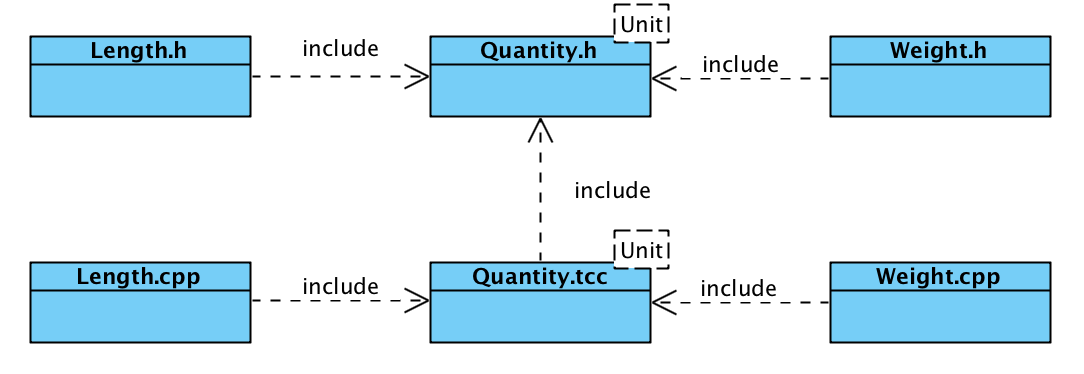
\includegraphics[width=0.8\textwidth]{figures/explict-template-inst.png}
\caption{显式模板实例化} 
 \label{fig:explict-template-inst}
\end{figure}



\begin{advise}
子类化优于\ascii{typedef}
\end{advise}

如果使用\ascii{typedef},如果存在对\ascii{Length}的依赖,即使是名字的声明依赖,除了包含头文件之外,别无选择。

另外,如果\ascii{Quantity}存在\ascii{virtual}函数时,\ascii{Length}还有进一步扩展\ascii{Quantity}的可能性,从而使设计提供了更大的灵活性。

反例:
\begin{leftbar}
\begin{c++}[caption={\ttfamily{quantity/Length.h}}]
#ifndef TYIW7364_JG6389457_BVGD7562_VNW12_JFH
#define TYIW7364_JG6389457_BVGD7562_VNW12_JFH

#include <quantity/Quantity.h>

struct LengthUnit;
typedef Quantity<LengthUnit> Length;

#endif
\end{c++}
\end{leftbar}

正例:
\begin{leftbar}
\begin{c++}[caption={\ttfamily{quantity/Length.h}}]
#ifndef TYIW7364_JG6389457_BVGD7562_VNW12_JFH
#define TYIW7364_JG6389457_BVGD7562_VNW12_JFH

#include <quantity/Quantity.h>

struct LengthUnit;
struct Length : Quantity<LengthUnit> {};

#endif
\end{c++}
\end{leftbar}

\end{content}
